\documentclass[conference]{IEEEtran}
\IEEEoverridecommandlockouts
% The preceding line is only needed to identify funding in the first footnote. If that is unneeded, please comment it out.
%Template version as of 6/27/2024

\usepackage{cite}
\usepackage{amsmath,amssymb,amsfonts}
\usepackage{algorithmic}
\usepackage{graphicx}
\usepackage{textcomp}
\usepackage{xcolor}
\usepackage{booktabs}
\usepackage{multirow}
\usepackage[caption=false,font=footnotesize]{subfig}
\def\BibTeX{{\rm B\kern-.05em{\sc i\kern-.025em b}\kern-.08em
    T\kern-.1667em\lower.7ex\hbox{E}\kern-.125emX}}
\begin{document}

% \title{AFGNN: Action Unit-Informed Facial-Audio Graph Network for Vlog-Based Depression Detection\thanks{This work is supported by the National Natural Science Foundation of China (No.62236006) and the Fundamental and Interdisciplinary Disciplines Breakthrough Plan of the Ministry of Education of China (JYB2025XDXM612). Corresponding author: Baobin Li (email: libb@ucas.ac.cn)}}
\title{AFGNN: Action Unit-Informed Facial-Audio Graph Network for Vlog-Based Depression Detection}


\author{
\IEEEauthorblockN{Anonymous Authors}
\IEEEauthorblockA{Anonymous Affiliations}
}
% \author{
% \IEEEauthorblockN{
% Tongqing Liu\IEEEauthorrefmark{1},
% Lihong Qiao\IEEEauthorrefmark{2},
% Tong Zhao\IEEEauthorrefmark{3},
% Baobin Li\IEEEauthorrefmark{1}
% }
% \IEEEauthorblockA{\IEEEauthorrefmark{1}School of Computer Science and Technology,
% 		University of Chinese Academy of Sciences, Beijing, China
% }

% \IEEEauthorblockA{
% \IEEEauthorrefmark{2}Chongqing University of Posts and Telecommunications, Chongqing, China
% }

% \IEEEauthorblockA{
% \IEEEauthorrefmark{3}School of Mathematical Sciences, University of Chinese Academy of Sciences, Beijing, China
% }
% }

\maketitle
\begin{abstract}
Vlog-based depression detection aims to identify depression-related behavioral patterns from naturalistic social-media videos. However, unconstrained vlog recordings often contain variations in facial visibility, speaking style, audio quality, and recording environment, making it difficult to capture structured facial-audio relations with sequential or global multimodal representations. This paper proposes an Action Unit-informed facial-audio graph network for this task. The proposed framework represents facial landmarks as an AU-informed spatio-temporal graph, where facial-topology edges model local facial action-related relations and temporal edges capture landmark motion. Acoustic descriptors are represented as an audio temporal graph to model short-term acoustic continuity. The two graph representations are encoded by modality-specific graph attention branches and integrated through bidirectional graph-level cross-modal gating. Experiments on D-Vlog show that the proposed method achieves an F1-score of 0.8077 and an AUC of 0.8041. Ablation studies further demonstrate the contributions of temporal edges, self-loops, velocity features, facial-audio combination, and graph-level gated fusion.
\end{abstract}

\begin{IEEEkeywords}
Depression detection, graph neural networks, multimodal fusion, cross-modal gating, D-Vlog.
\end{IEEEkeywords}

\section{Introduction}
\label{sec:intro}
Depression is a common mental health disorder that affects emotional well-being, social functioning, and daily activities. Conventional depression screening and assessment usually rely on clinical interviews and self-report questionnaires, which may be affected by reporting bias, response burden, and unequal access to mental health resources. These limitations have motivated computational detection from observable behavioral signals. Among such signals, facial behavior and acoustic patterns are widely studied because depression-related states may be reflected in reduced facial expressiveness, psychomotor changes, and altered vocal prosody~\cite{cohn2009detecting,cummins2015review,yang2013vocal}.

Audio-visual depression detection has been widely studied in interview-based settings. Benchmarks such as AVEC and DAIC-WOZ provide controlled protocols for analyzing facial behavior, head movement, speech, and language in depression assessment~\cite{valstar2014avec,gratch2014daic,ringeval2017avec}. Recent multimodal datasets have further broadened this setting to more diverse recording conditions~\cite{zou2023cmdc,uddin2023deep}. In contrast,  user-generated vlogs capture facial and acoustic behaviors in less constrained social-media environments. D-Vlog and LMVD are representative vlog-based datasets for studying depression-related behaviors in social-media videos~\cite{yoon2022dvlog,he2024lmvd}.
However, vlog recordings are substantially less controlled than interview videos, with large variations in facial visibility, speaking style, audio quality, recording environment, and background context. Such variability makes it difficult to rely only on frame-level sequences or global multimodal features, and motivates structured behavioral representations that explicitly model the organization of facial and acoustic behavior.

To handle the variability of audio-visual behavior in vlog recordings, recent studies have improved temporal representation learning and multimodal fusion for depression detection. Representative methods have explored time-aware attention, spatio-temporal transformers, Mamba-based sequence encoders, temporal-difference attention, and cross-modal fusion to capture behavioral dynamics and modality complementarity~\cite{model:TAMFN,tao2024depmstat,xing2024emomamba,liu2024mddmamba,hu2024sedcfn,jia2024bmbrt,zhang2024mtdan,zhao2025decoupled}.
Graph-based representations have also been introduced for video-based depression recognition, suggesting that structural relations may provide useful information beyond  sequential features~\cite{xu2025twostage}. 
For instance, temporal graph neural networks have been used to model non-contiguous spatiotemporal dependencies in facial behavior~\cite{model:MSI-Net}. 
However, these methods mainly focus on temporal encoding or multimodal integration, while facial action-related organization of landmarks  remains insufficiently explored. 
In particular, facial landmarks are often treated as coordinate sequences, visual features, or generic spatio-temporal inputs, rather than as structured action-related representations.

This issue is particularly important for geometry-based facial representation. Facial landmarks are not isolated coordinate points but are organized around facial action-related regions, including the eyebrows, eyes, nose, mouth, and facial contour. 
These regions are closely associated with local facial actions described by the Facial Action Coding System (FACS), in which Action Units provide a standard description of visible facial muscle movements~\cite{ekman1978facs,baltrusaitis2016openface,baltrusaitis2018openface}.  
Recent work has also explored statistically significant Action Units as covariates to guide graph attention for depression recognition~\cite{zhao2026covariate}.
In vlog-based depression datasets, explicit AU annotations or AU intensity labels are often unavailable. Accordingly, this work adopts an AU-informed rather than AU-annotated graph design. The proposed graph does not use AU labels as supervision; instead, it organizes landmark positions and motion according to facial action-related regions, forming a structured representation of facial topology and temporal movement.


\begin{figure*}[t!]
\centering
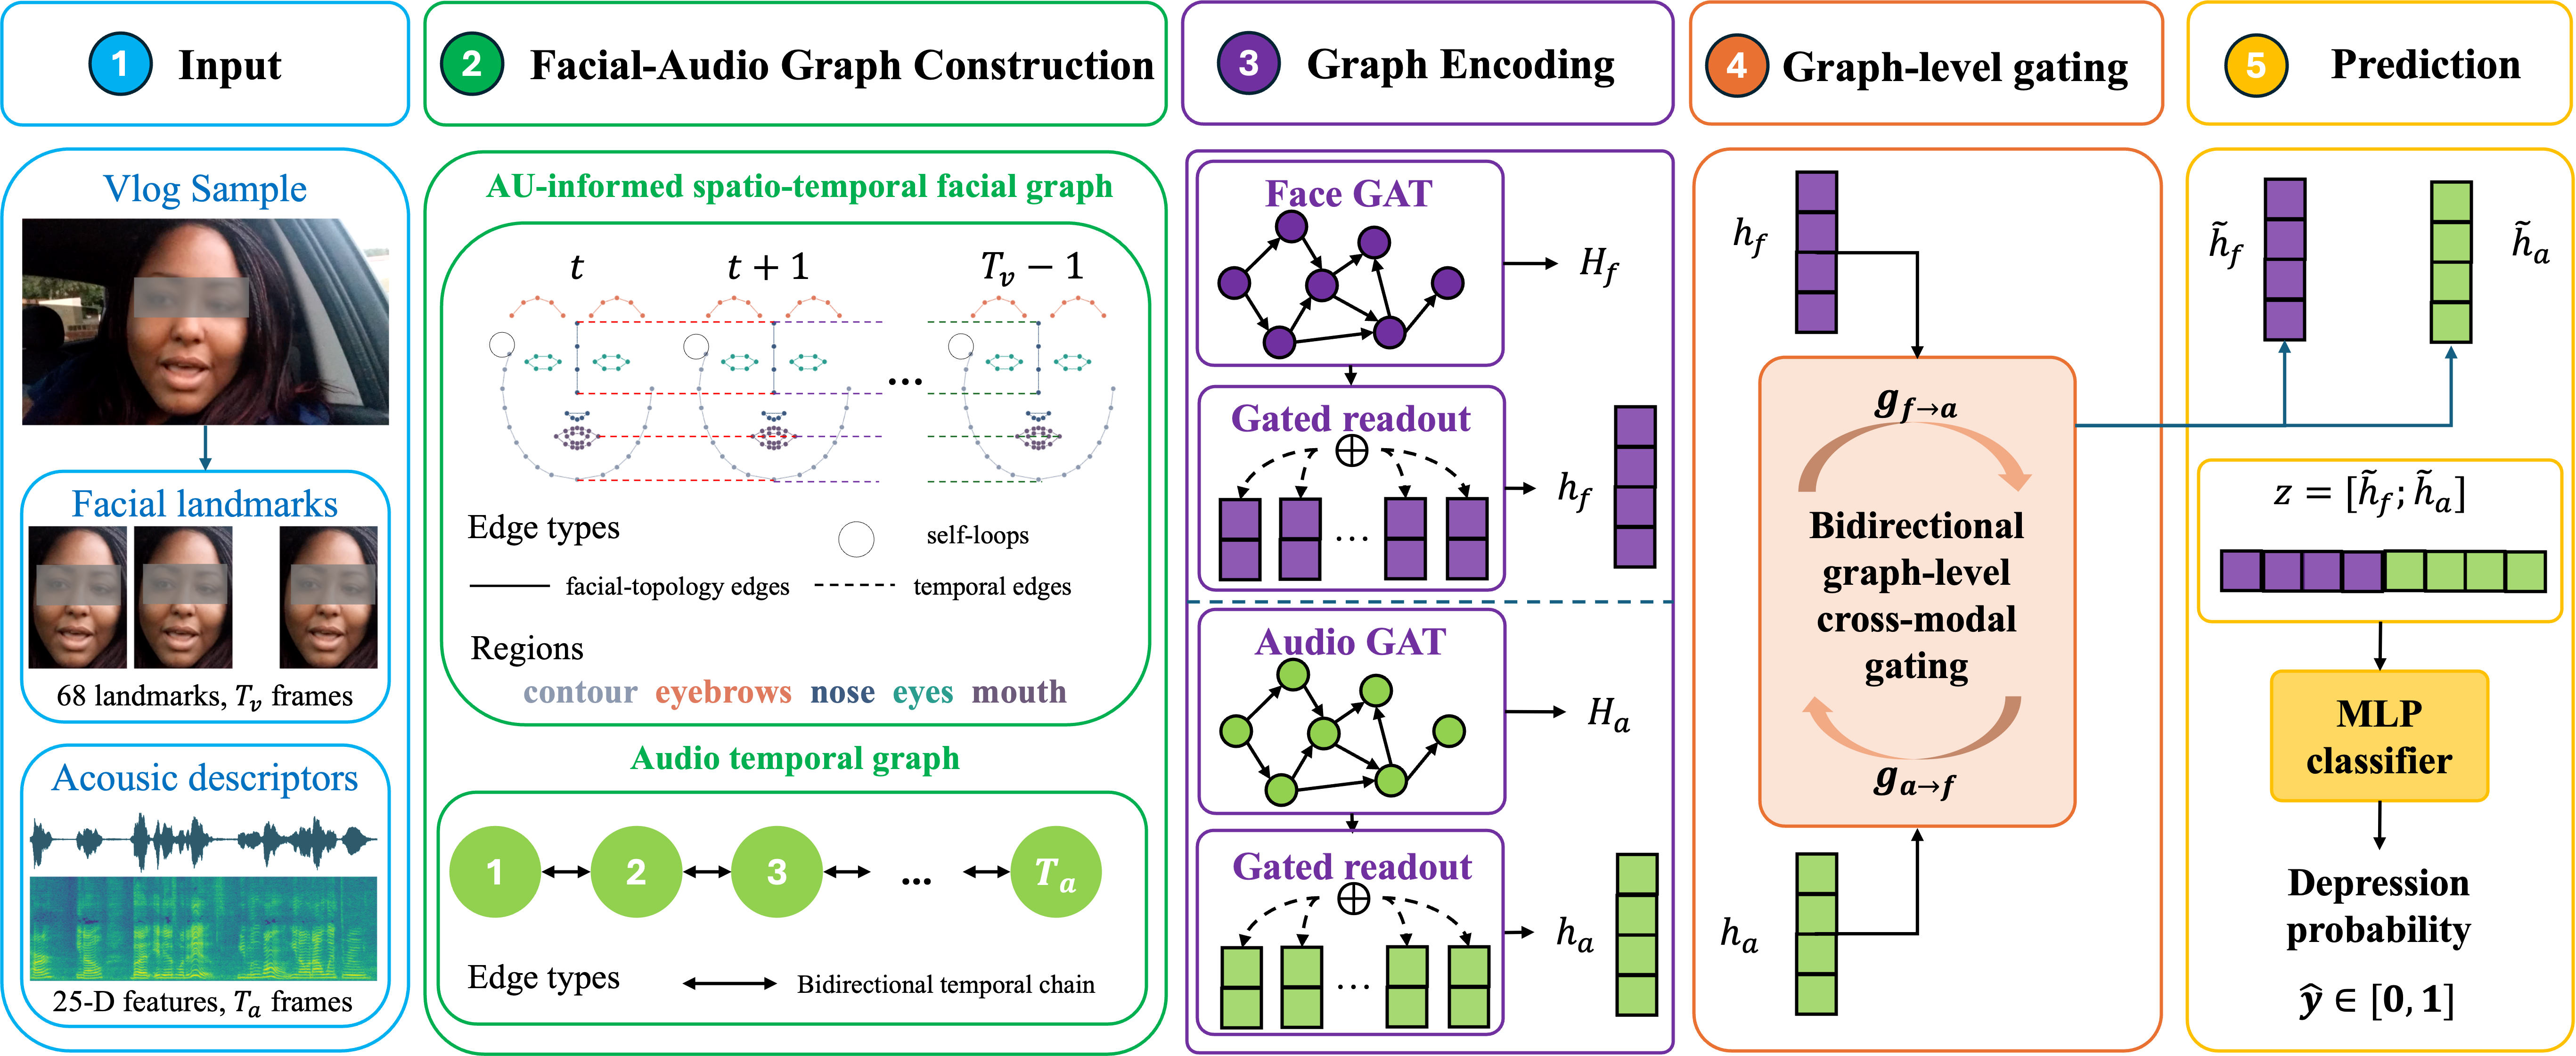
\includegraphics[width=0.96\textwidth]{Framework.png} 
\caption{Overall framework of AFGNN. Facial landmarks are represented as an AU-informed spatio-temporal facial graph with facial-topology edges, temporal edges, region-aware node features, and self-loops. Acoustic descriptors are represented as an audio temporal graph. The two graphs are encoded by lightweight GAT branches and integrated through bidirectional graph-level cross-modal gating for depression prediction.}
\label{fig:framework}
\end{figure*}

Graph networks provide a natural way to model such structured facial representations by treating landmarks as nodes and spatial-temporal relations as edges. Prior studies on facial expression recognition and AU recognition have shown that graph-based relational reasoning is useful for modeling dependencies among facial regions, landmarks, or action units~\cite{song2021uncertain,ge2024mgrr,liao2022fergcn}. However, these studies mainly target facial expression or AU recognition rather than vlog-based depression detection. In this task, facial actions are often subtle, temporally evolving, and coupled with acoustic behavior. 
Therefore, an effective representation should jointly encode AU-informed facial topology, landmark motion, and acoustic information, as also explored by recent audio-visual graph learning frameworks~\cite{li2025avsgnn}. This motivates a unified facial-audio graph network that combines facial-topology structure, temporal facial dynamics, and audio temporal relations.

To address these issues, we propose AFGNN, an Action Unit-informed Facial-Audio Graph Network for vlog-based depression detection. The proposed framework organizes facial landmarks into an AU-informed spatio-temporal facial graph, where intra-frame facial-topology edges encode local relations within facial action-related regions and inter-frame temporal edges capture landmark motion. Acoustic descriptors are represented as an audio temporal graph to model short-term acoustic continuity. The facial and audio graphs are encoded by lightweight graph attention branches and integrated through bidirectional graph-level cross-modal gating. This design provides a structured representation that combines facial action-related topology, landmark motion, acoustic temporal relations, and cross-modal interaction.

The main contributions of this work are summarized as follows:

\begin{itemize}
\item This study formulates vlog-based depression detection as an Action Unit-informed facial-audio graph learning problem, emphasizing structured modeling of landmark-level facial action organization.

\item The proposed framework constructs an AU-informed spatio-temporal facial graph and an audio temporal graph, and integrates them through bidirectional graph-level cross-modal gating.


\item Experiments on D-Vlog show that the proposed method achieves an F1-score of 0.8077 and an AUC of 0.8041. Ablation studies further show that temporal edges, self-loops, velocity features, facial-audio combination, and graph-level gated fusion contribute to performance.
\end{itemize}


\section{AU-Informed Facial-Audio Graph Network}
\label{sec:method}
This section presents the proposed AU-informed facial-audio graph network. We first describe the overall architecture, then introduce facial and audio graph construction, and finally present graph encoding and graph-level cross-modal gating.

\subsection{Overall Framework}

As shown in Fig.~\ref{fig:framework}, each vlog sample is represented by a facial landmark sequence and an acoustic descriptor sequence,
\begin{equation}
P \in \mathbb{R}^{T_v \times 68 \times 2}, \quad
A \in \mathbb{R}^{T_a \times d_a},
\end{equation}
where \(T_v\) and \(T_a\) denote the visual and acoustic sequence lengths, respectively, and \(d_a=25\) in our implementation. The objective is to predict a binary depression label \(y \in \{0,1\}\).

The proposed framework maps the two input sequences into an AU-informed spatio-temporal facial graph and an audio temporal graph,
\begin{equation}
G_f = (V_f, E_f, X_f), \quad
G_a = (V_a, E_a, X_a),
\end{equation}
where \(V_m\), \(E_m\), and \(X_m\) denote the nodes, edges, and node features of modality \(m \in \{f,a\}\). After modality-specific graph attention encoding and graph-level cross-modal gating, the final prediction is obtained as
\begin{equation}
z = [\tilde{h}_f; \tilde{h}_a], \quad
\hat{y} = \sigma(\mathrm{MLP}(z)),
\end{equation}
where \(\tilde{h}_f\) and \(\tilde{h}_a\) denote the gated facial and audio graph-level representations.


\subsection{Facial and Audio Graph Construction}

The facial graph is constructed from sampled landmark coordinates. Each node \(v^f_{i,t} \in V_f\) represents landmark \(i\) at visual frame \(t\). Its feature vector concatenates landmark position, frame-wise displacement, and facial-region identity
\begin{equation}
x^f_{i,t} = [p_{i,t}; \Delta p_{i,t}; r_i] \in \mathbb{R}^{13}, \quad
\Delta p_{i,t} =
\begin{cases}
p_{i,t} - p_{i,t-1}, & t > 1, \\
0, & t = 1,
\end{cases}
\end{equation}
where \(p_{i,t} \in \mathbb{R}^{2}\) denotes the landmark coordinate and \(r_i \in \{0,1\}^{9}\) denotes the facial-region identity of landmark \(i\). The nine regions include the face contour, left eyebrow, right eyebrow, nose bridge, nose bottom, left eye, right eye, outer mouth, and inner mouth. Thus, \(|V_f| = 68T_v\) and \(X_f \in \mathbb{R}^{68T_v \times 13}\).

The facial edge set consists of intra-frame facial-topology edges, inter-frame temporal edges, and self-loops
\begin{equation}
E_f = E_{\mathrm{top}} \cup E_{\mathrm{temp}} \cup E_{\mathrm{self}}.
\end{equation}
The facial-topology edges \(E_{\mathrm{top}}\) are derived from the standard 68-point landmark layout. They connect adjacent landmarks within facial action-related regions, using chain connections for open components and ring connections for closed components. The temporal edges connect the same landmark across consecutive frames, and self-loops preserve node-specific information during message passing
\begin{equation}
E_{\mathrm{temp}} =
\{(v^f_{i,t}, v^f_{i,t+1}), (v^f_{i,t+1}, v^f_{i,t})\},
\quad
E_{\mathrm{self}} = \{(v^f_{i,t}, v^f_{i,t})\}.
\end{equation}
Here, \(E_{\mathrm{temp}}\) is defined for \(i=1,\ldots,68\) and \(t=1,\ldots,T_v-1\), while \(E_{\mathrm{self}}\) is defined for all facial nodes. This construction yields an AU-informed spatio-temporal facial graph that organizes landmark motion according to facial action-related topology without requiring AU annotations.

The audio graph is constructed from sampled acoustic descriptors. Each node \(v^a_t \in V_a\) corresponds to one acoustic frame, and its feature is the standardized acoustic descriptor
\begin{equation}
x^a_t = \tilde{a}_t = \frac{a_t - \mu}{\sigma + \epsilon}, \quad
X_a \in \mathbb{R}^{T_a \times d_a},
\end{equation}
where \(\mu,\sigma \in \mathbb{R}^{d_a}\) are computed from the training set and applied to the validation and test sets. The audio edge set is defined as a bidirectional temporal chain
\begin{equation}
E_a =
\{(v^a_t, v^a_{t+1}), (v^a_{t+1}, v^a_t)
\mid t = 1,\ldots,T_a-1\}.
\end{equation}
This lightweight structure models short-term temporal continuity among acoustic descriptors. 











\subsection{Graph Encoding and Gated Fusion}

The facial and audio graphs are encoded by modality-specific graph attention branches:
\begin{equation}
\mathbf{H}_m = \mathrm{GAT}_m(G_m)
= \{\mathbf{h}^m_u \mid u \in V_m\}, \quad
\mathbf{h}^m_u \in \mathbb{R}^{d_m}.
\end{equation}
Here, \(h^m_u\) denotes the node representation of node \(u\) in modality \(m\in \{f,a\}\).

A gated readout is then used to aggregate node representations into a graph-level embedding. For each node \(u\), a modality-specific gate network produces an unnormalized score, which is normalized over all nodes in the graph
\begin{equation}
\beta^m_u =
\frac{\exp(g_m(h^m_u))}
{\sum_{v \in V_m}\exp(g_m(h^m_v))},
\quad
h_m = \sum_{u \in V_m} \beta^m_u h^m_u .
\end{equation}
where \(\beta^m_u\) denotes the readout weight of node \(u\), and \(h_m\) is the graph-level embedding of modality \(m\).

Since each modality is summarized into a single graph-level embedding, the proposed framework adopts graph-level gating rather than token-level cross-attention. For \(m \in \{f,a\}\), let
\begin{equation}
q_m = W^m_q h_m, \quad k_m = W^m_k h_m .
\end{equation}
The directional gates and residual updates are defined as
\begin{equation}
g_{f \leftarrow a}
=
\sigma\left(\frac{q_f^\top k_a}{\sqrt{d_g}}\right),
\quad
\tilde{h}_f
=
h_f + g_{f \leftarrow a} W^{a \rightarrow f}_v h_a,
\end{equation}
\begin{equation}
g_{a \leftarrow f}
=
\sigma\left(\frac{q_a^\top k_f}{\sqrt{d_g}}\right),
\quad
\tilde{h}_a
=
h_a + g_{a \leftarrow f} W^{f \rightarrow a}_v h_f .
\end{equation}
Here, \(W^{a \rightarrow f}_v \in \mathbb{R}^{d_f \times d_a}\) and
\(W^{f \rightarrow a}_v \in \mathbb{R}^{d_a \times d_f}\) project the graph-level embedding of one modality into the feature space of the other modality before residual updating. 

The model is optimized with focal loss
\begin{equation}
\mathcal{L}_{\mathrm{focal}}
=
-\alpha_t(1-p_t)^\gamma \log(p_t),
\end{equation}
\begin{equation}
p_t = y\hat{y} + (1-y)(1-\hat{y}),
\quad
\alpha_t = \alpha y + (1-\alpha)(1-y),
\end{equation}
where \(p_t\) is the predicted probability of the ground-truth class. We set \(\alpha=0.25\) and \(\gamma=2\). The validation set is used for checkpoint selection and decision-threshold determination.

During inference, \(K\) independently trained models are averaged at the probability level 
$\hat{y}_{\mathrm{ens}}
=
\frac{1}{K}
\sum_{k=1}^{K} \hat{y}^{(k)} .
$
% \begin{equation}
% \hat{y}_{\mathrm{ens}}
% =
% \frac{1}{K}
% \sum_{k=1}^{K} \hat{y}^{(k)} .
% \end{equation}
In this work, \(K=3\) for final ensemble inference.






\section{Experiments}
\label{sec:experiments}
This section evaluates the proposed framework on D-Vlog through comparison with existing reported methods, ablation studies, and visualization-based analysis. The evaluation examines the effects of graph construction, modality combination, gated fusion, and inference design.

\subsection{Experimental Setup}

Experiments are conducted on the public D-Vlog dataset~\cite{yoon2022dvlog}, which contains 961 vlogs from 816 individuals, including 555 depressed samples and 406 control samples. Following the official split, the dataset is divided into 647 training samples, 102 validation samples, and 212 test samples with a ratio of 7:1:2, as summarized in Table~\ref{tab:dataset}.

\begin{table}[htb]
\centering
\caption{D-Vlog dataset statistics.}
\label{tab:dataset}
\begin{tabular}{lccc}
\toprule[1.2pt]
Split & Total & Depressed & Control \\
\midrule[0.8pt]
Train & 647 & 373 & 274 \\
Validation & 102 & 57 & 45 \\
Test & 212 & 125 & 87 \\
\bottomrule[1.2pt]
\end{tabular}
\end{table}

Each sample is represented by pre-extracted facial landmarks and acoustic descriptors. The visual input consists of 68 facial landmarks, and the acoustic input consists of 25-dimensional openSMILE descriptors. Since the proposed framework uses only landmark coordinates and acoustic descriptors, no raw facial pixels or identifiable facial images are processed in this study. Performance is evaluated using Accuracy, Precision, Recall, F1-score, and Area Under the ROC Curve. The held-out test set is used only for final evaluation, while the validation set is used for checkpoint selection and threshold calibration.

All experiments are implemented with PyTorch Geometric~\cite{fey2019fast}. The facial graph uses \(T_v=32\) sampled visual frames, and the audio graph uses \(T_a=32\) acoustic frames. The facial GAT branch contains three layers with hidden dimension 128 and four attention heads, while the audio GAT branch contains two layers with hidden dimension 64 and four attention heads. Dropout is set to 0.3. The framework is trained with Adam using a learning rate of \(10^{-3}\), weight decay of \(10^{-4}\), and a batch size of 32. Training lasts up to 100 epochs, with early stopping based on validation AUC and a patience of 15 epochs. A ReduceLROnPlateau scheduler reduces the learning rate by a factor of 0.5 if validation AUC does not improve for 5 consecutive epochs, and gradient clipping is applied with a maximum norm of 1.0. The final model contains approximately \(1.2 \times 10^5\) trainable parameters.

Unless otherwise specified, ablation results are reported using a single model without ensemble inference. The final test result is obtained by averaging three independently trained models at the probability level.

\subsection{Comparison with Existing Methods}

Table~\ref{tab:comparison} compares the proposed method with existing methods reported on D-Vlog. The proposed method achieves an accuracy of 0.7642 and an F1-score of 0.8077, both of which are higher than those of the listed methods with reported values. These results suggest that organizing facial landmarks and acoustic descriptors into structured graph representations is effective for vlog-based depression detection.

It should be noted that the reported results are not always obtained under identical evaluation protocols. Some methods report results using five-fold cross-validation, whereas this study follows the official train, validation, and test split. Therefore, the comparison is intended to provide a reference against reported D-Vlog results rather than a strictly controlled re-implementation comparison.




\begin{table}[t]
\centering
\caption{Comparison with existing methods reported on D-Vlog.}
\label{tab:comparison}
\begin{tabular}{lcccc}
\hline
Method & Acc & Prec & Rec & F1 \\
\hline
TAMFN~\cite{model:TAMFN} & -- & 0.6602 & 0.6650 & 0.6582 \\
STST~\cite{model:STST} & 0.7070 & 0.7250 & 0.7767 & 0.7500 \\
MDAVIF~\cite{model:MDAVIF} & -- & 0.7425 & 0.7600 & 0.7525 \\
DepMamba~\cite{model:DepMamba} & 0.6887 & 0.6819 & \textbf{0.8699} & 0.7644 \\
AttMamba~\cite{model:AttMamba} & 0.6940 & 0.7029 & 0.8066 & 0.7552 \\
DepMSTAT~\cite{tao2024depmstat} & -- & 0.7153 & 0.7560 & 0.7351 \\
ASYM~\cite{model:ASYM} & 0.7468 & 0.7387 & 0.7619 & 0.7490 \\
MSTGT~\cite{model:MSTGT} & 0.7138 & 0.7247 & 0.8428 & 0.7681 \\
MSI-Net~\cite{model:MSI-Net} & 0.7025 & \textbf{0.7891} & 0.6963 & 0.7391 \\
AFGNN (Ours) & \textbf{0.7642} & 0.7664 & 0.8537 & \textbf{0.8077} \\
\hline
\end{tabular}
\end{table}


\begin{table}[t]
\centering
\caption{Component-level ablation on facial graph structure. All variants keep the audio branch and graph-level gated fusion unchanged. The full model includes facial-topology edges, temporal edges, facial-region encoding, velocity features, and self-loops.}
\label{tab:face_ablation}
\footnotesize
\setlength{\tabcolsep}{6pt}
\begin{tabular}{lcc}
\hline
Configuration & F1 & AUC \\
\hline
Full model & \textbf{0.794} & \textbf{0.802} \\
\hline
Remove Facial-topology edges & 0.786 & 0.792 \\
Remove Temporal edges & 0.748 & 0.763 \\
Remove Region encoding & 0.789 & 0.786 \\
Remove Velocity features & 0.752 & 0.760 \\
Remove Self-loop & 0.748 & 0.778 \\
\hline
Add Dynamic edges $(k=1)$ & 0.714 & 0.672 \\
Motion-based edges $(k=2)$ & 0.709 & 0.664 \\
\hline
\end{tabular}
\end{table}



% \begin{table}[t]
% \centering
% \caption{Component-level ablation on facial graph structure. All variants keep the audio branch and graph-level gated fusion unchanged. The
% full model uses facial-topology edges, temporal edges,facial-region encoding, velocity features, and self-loops.}
% \label{tab:graph_ablation}
% \small
% \begin{tabular}{lcc}
% \toprule[1.2pt]
% Facegraphconfiguration&F1&AUC\\
% \midrule[0.8pt]
% Full(Topology+Temporal+Region+Velocity+Self-loop)&\textbf{0.794}&\textbf{0.802}\\
% \midrule[0.8pt]
% Topology edges&0.786&0.792\\
% Temporaledges&0.748&0.763\\
% Regionone-hot&0.789&0.786\\
% Velocity$[dx,dy]$&0.752&0.760\\
% Self-loop&0.748&0.778\\
% \midrule[0.8pt]
% Static+Temporal+Dynamic($k$=1)&0.714&0.672\\
% Motion+Region($k$=2)&0.709&0.664\\
% \bottomrule[1.2pt]
% \end{tabular}
% \end{table}

\begin{figure}[t]
\centering
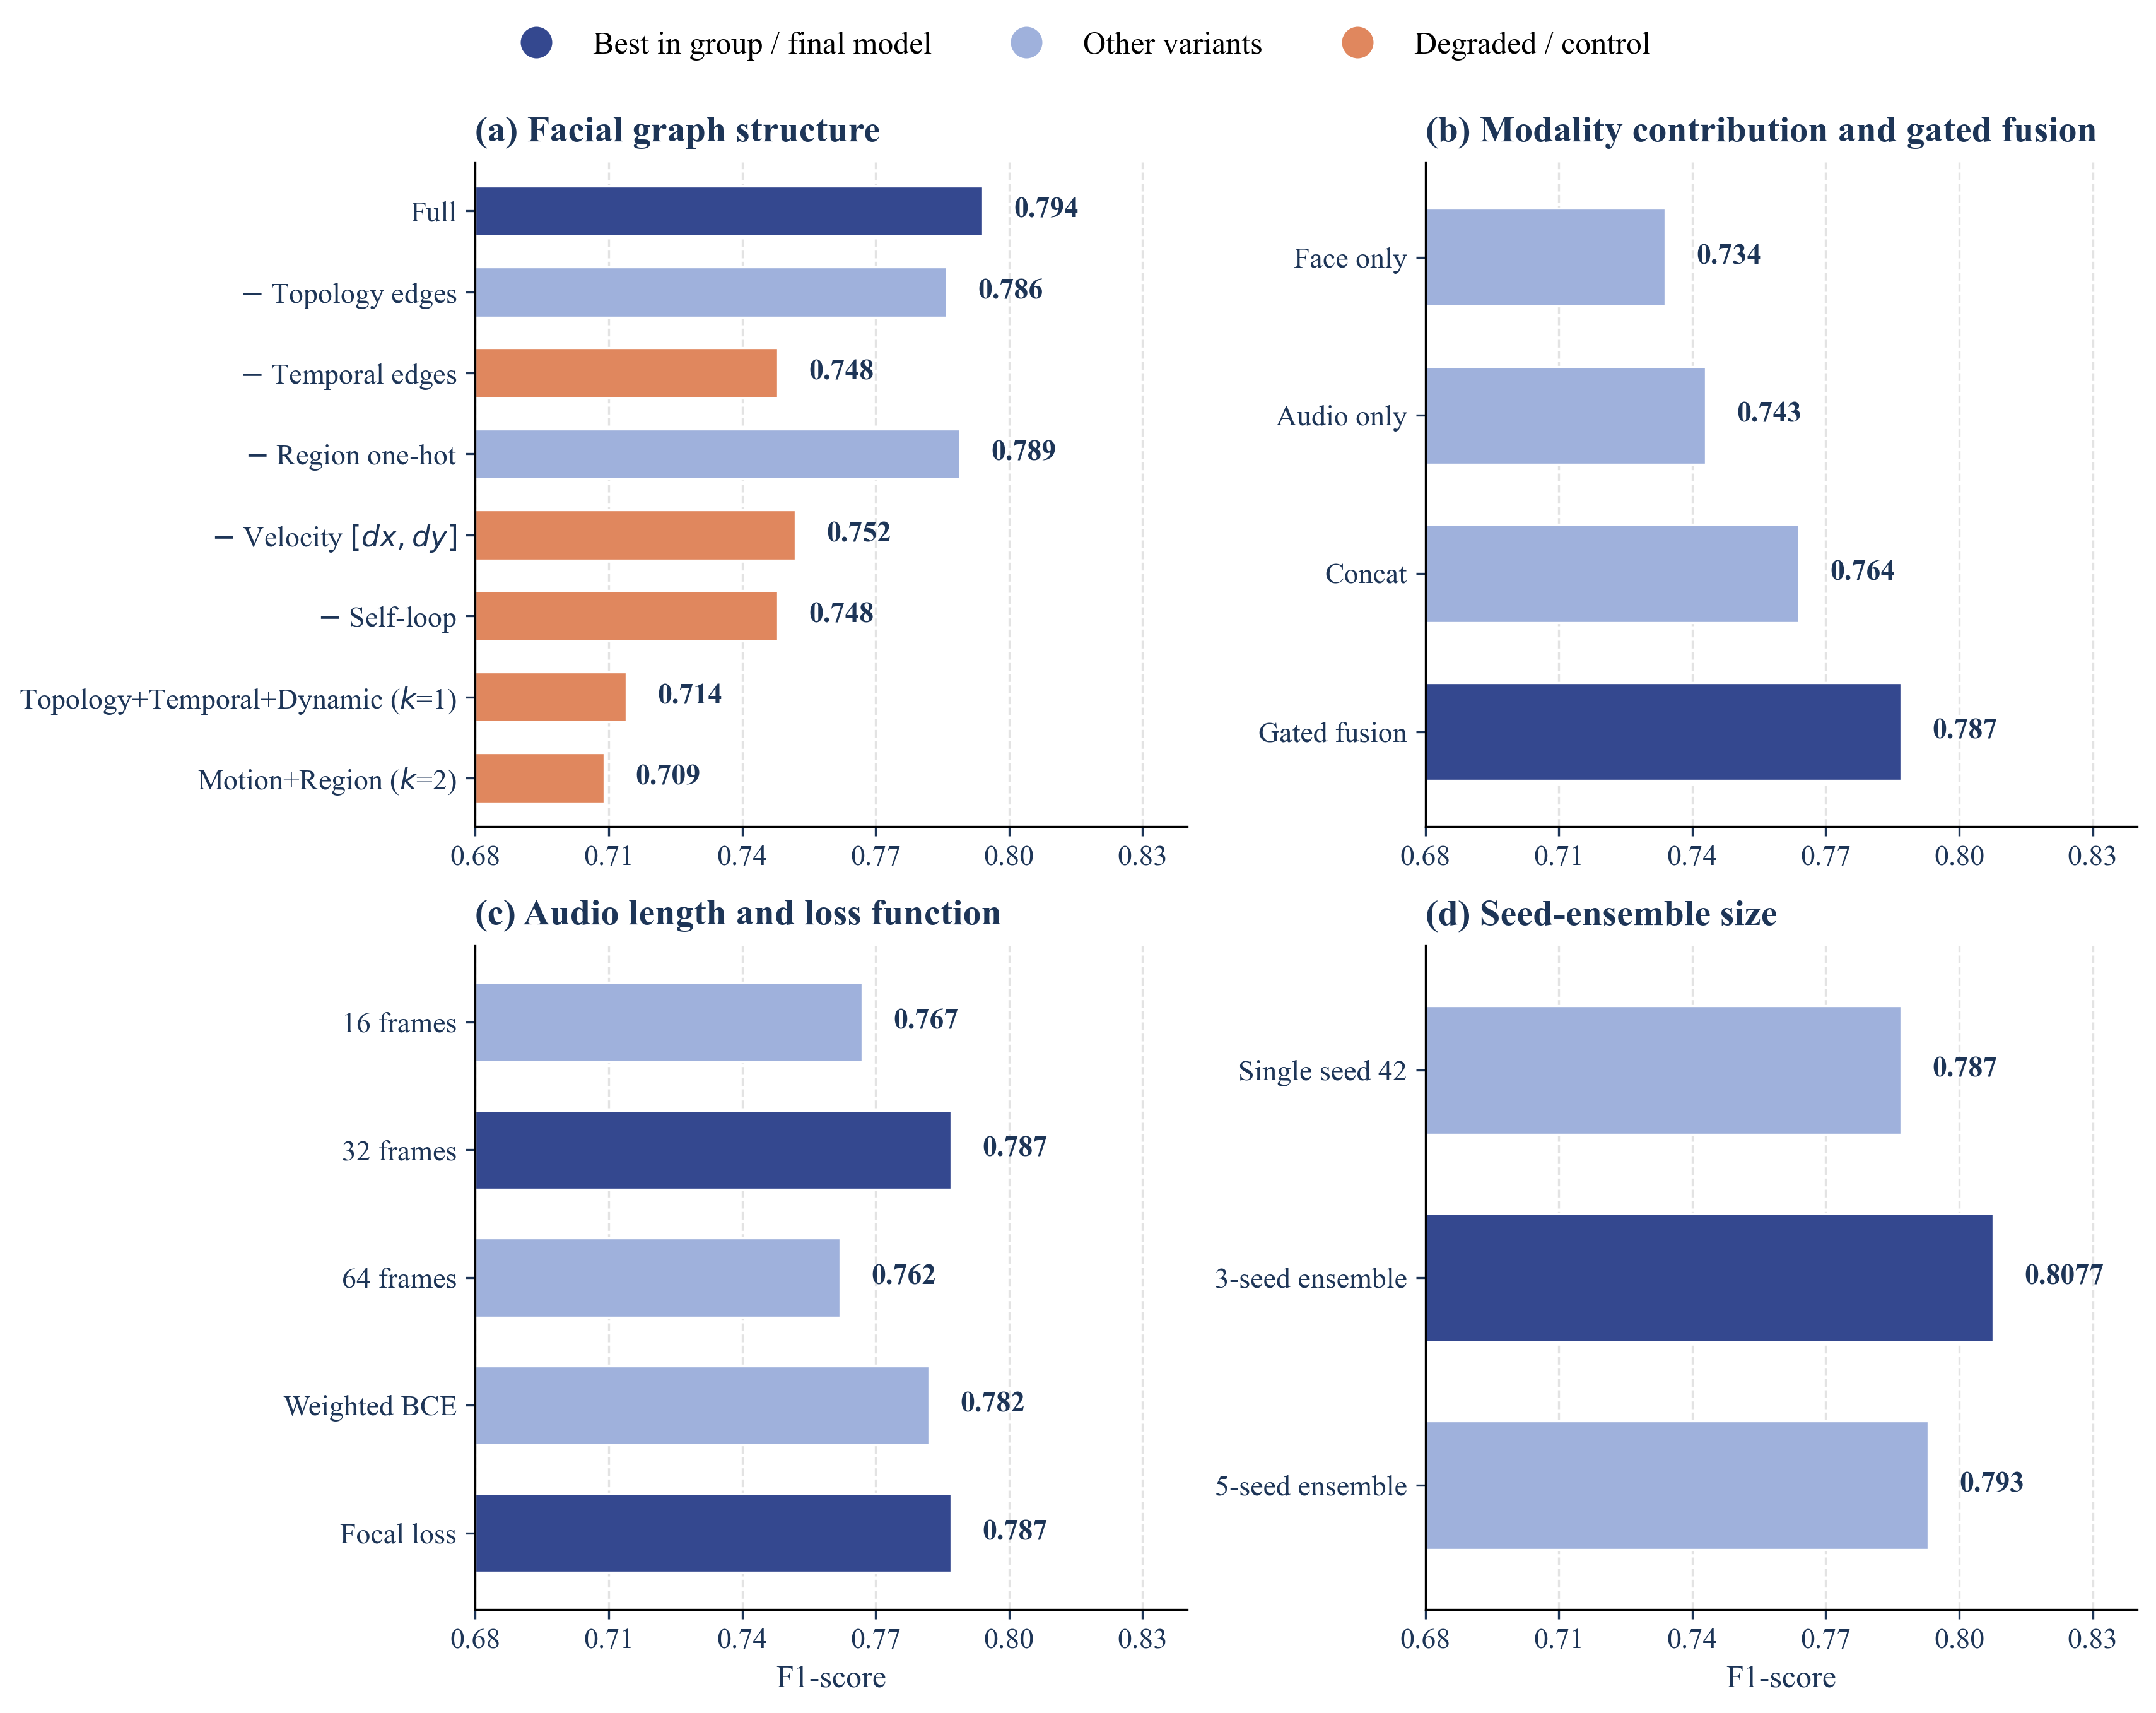
\includegraphics[width=\linewidth]{Ablation results.png}
\caption{Visualization of the main ablation results. (a) Facial graph structure. (b) Modality contribution and gated fusion. (c) Audio length and loss function. (d) Seed-ensemble size.}
\label{fig:ablation}
\end{figure}


\begin{figure*}[t]
\centering
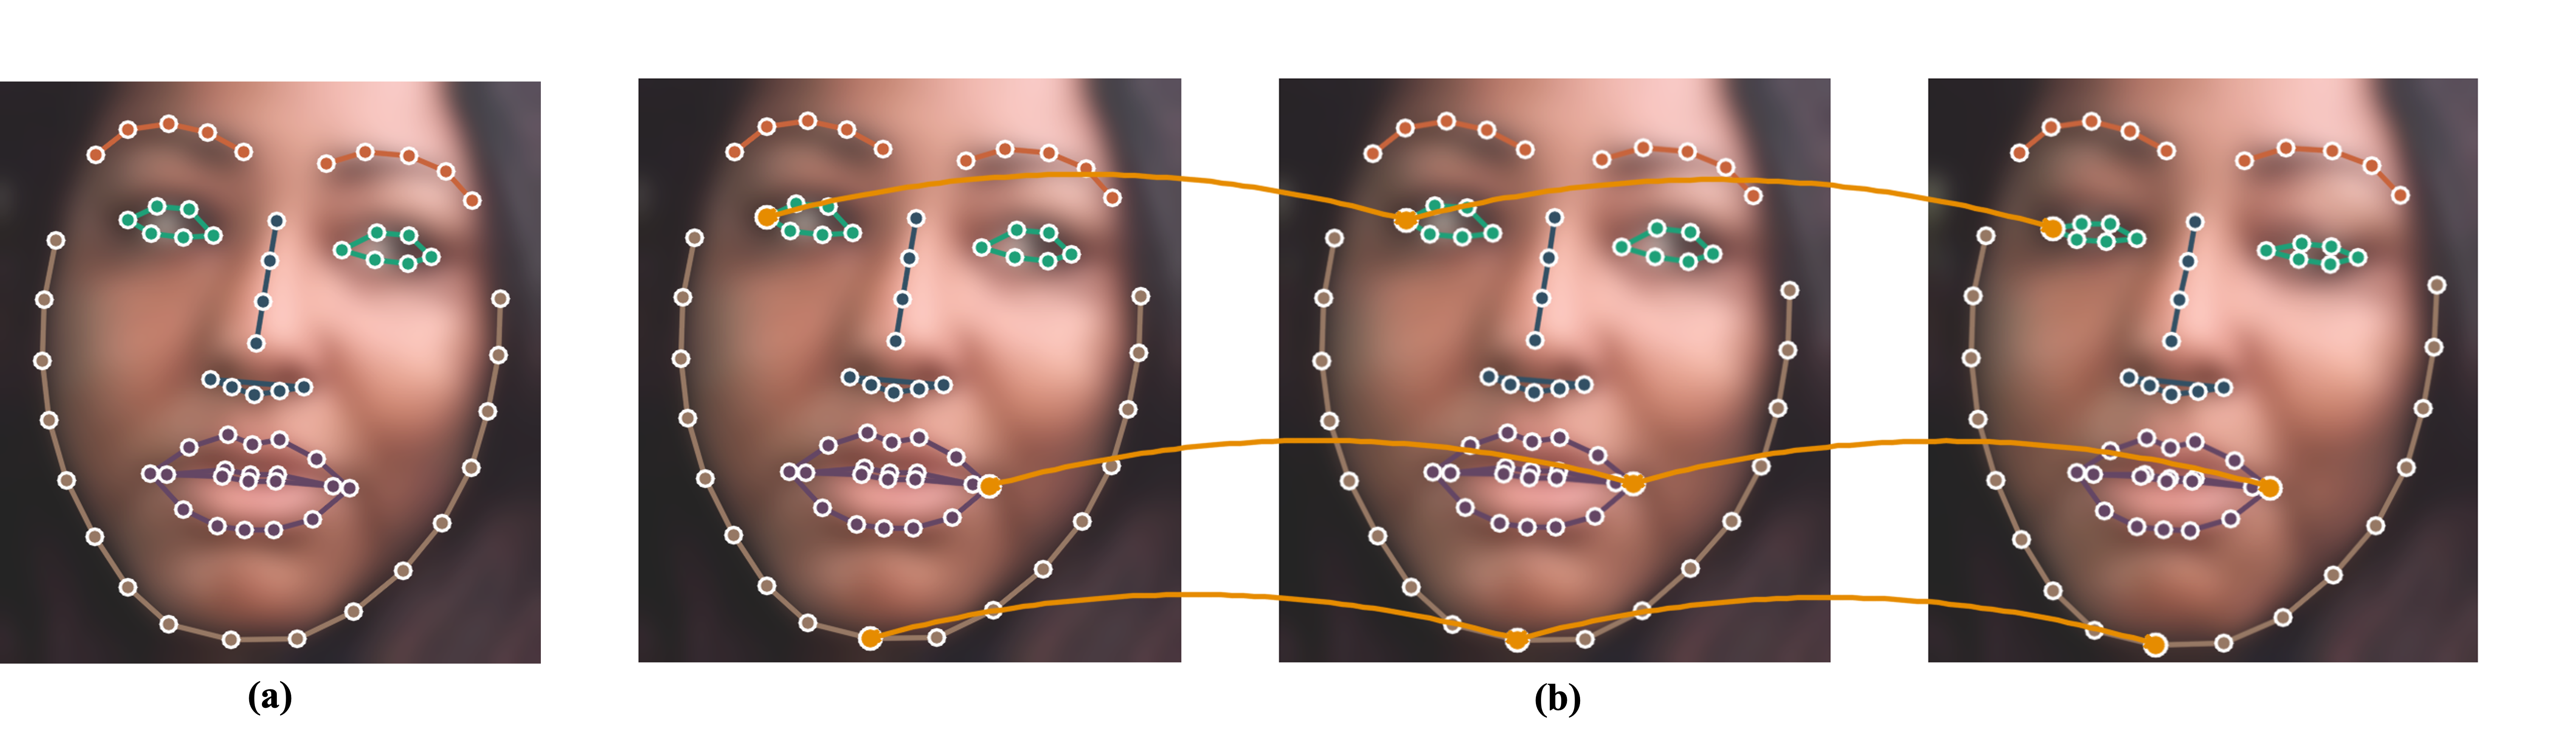
\includegraphics[width=\textwidth]{Face graph.png}
\caption{AU-informed facial graph construction. (a) The 68-point landmark topology overlaid on the face, colored by facial action-related region. (b) Temporal edges connect the same landmark across consecutive frames.}
\label{fig:face_graph}
\end{figure*}


\begin{figure*}[t]
\centering
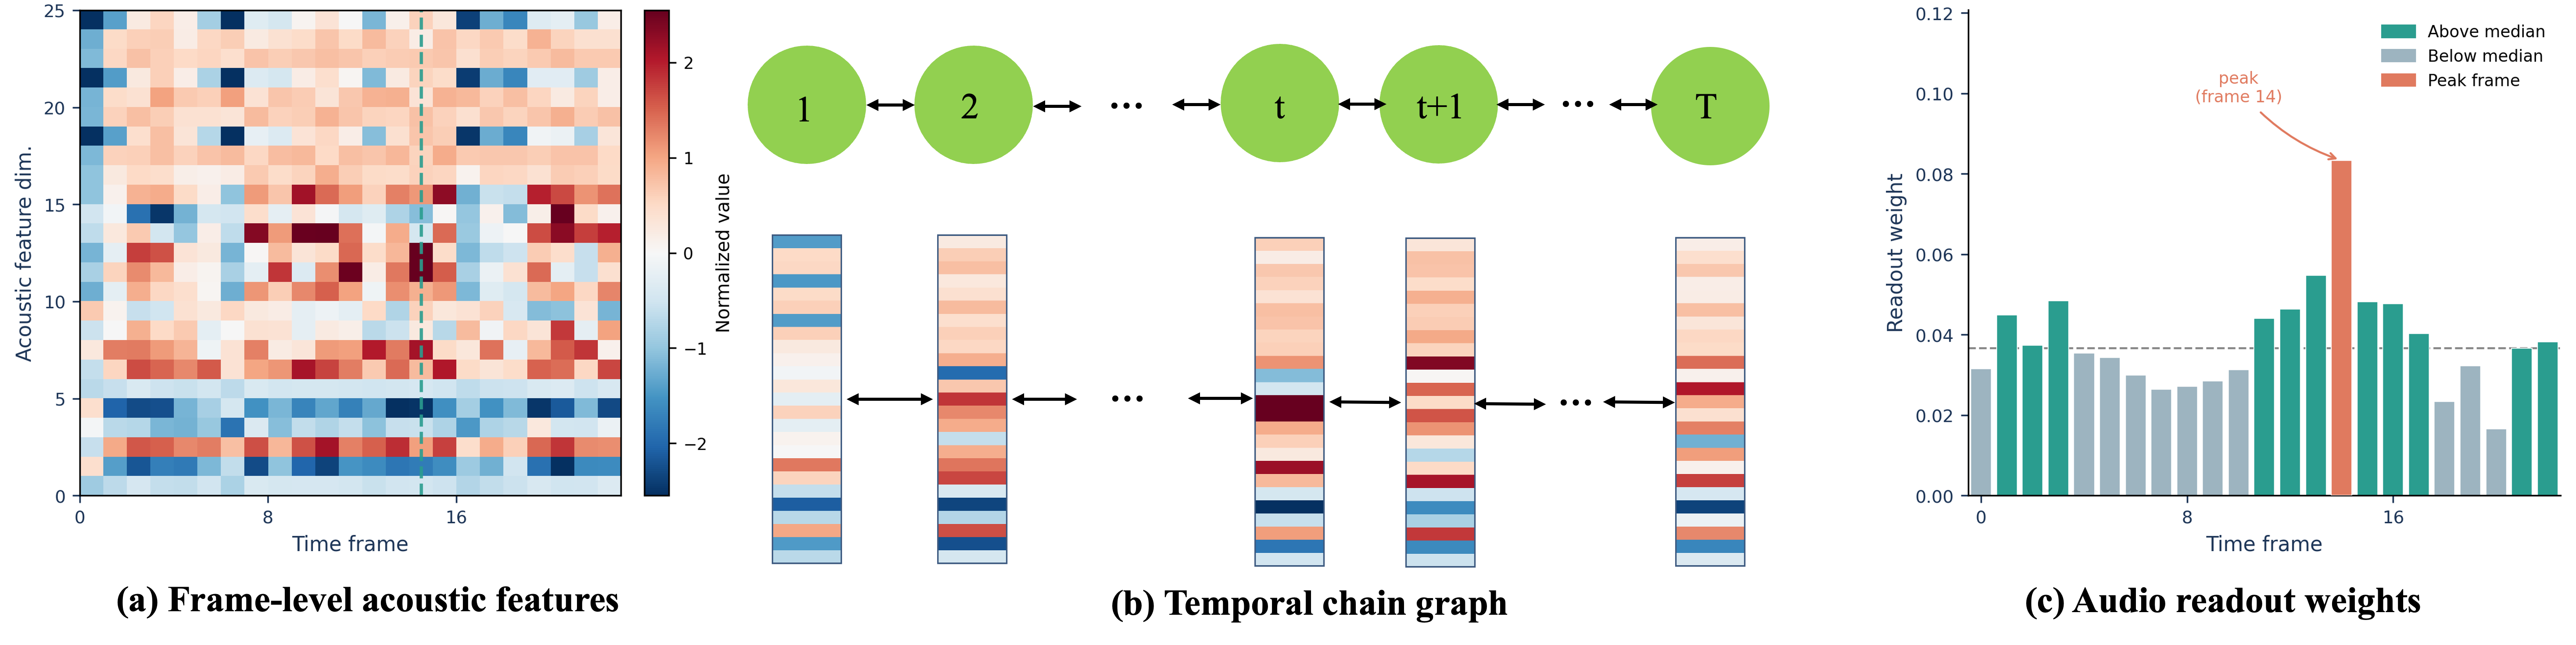
\includegraphics[width=0.98\linewidth]{Audio graph.png}
\caption{Audio graph construction. (a) Frame-level acoustic feature sequence. (b) The temporal chain graph connects adjacent time frames bidirectionally. (c) Example readout weights; higher weights indicate frames that contribute more strongly to the graph-level audio representation.}
\label{fig:audio_graph}
\end{figure*}




\subsection{Ablation Study}

Ablation studies are conducted to examine how the main components of the proposed framework contribute to performance. The analysis covers four aspects: facial graph structure, modality contribution and gated fusion, training and inference design, and facial-region sensitivity. The numerical results are reported in Tables~\ref{tab:face_ablation}--\ref{tab:region_ablation}, and the main ablation trends are visualized in Fig.~\ref{fig:ablation}.

\textit{Graph structure.}
Table~\ref{tab:face_ablation} evaluates the contribution of facial graph components while keeping the audio branch and graph-level gated fusion unchanged. For the dynamic graph baselines, frame-level \(k\)-nearest-neighbor edges are added to the facial graph:
\begin{equation}
\mathcal{N}^{\mathrm{dyn}}_k(v^f_{i,t})
=
\mathrm{TopK}_{j \ne i}\,
\mathrm{sim}(s_{i,t}, s_{j,t}),
\end{equation}
where \(s_{i,t}\) is set to \(x^f_{i,t}\) for feature-similarity graphs and to \(\Delta p_{i,t}\) for motion-consistency graphs. These dynamic edges are used only for ablation and are not included in the final configuration.

The full facial graph achieves the best performance, with an F1-score of 0.794 and an AUC of 0.802. Removing temporal edges, velocity features, or self-loops leads to larger F1-score reductions, indicating that temporal continuity, landmark motion, and node-specific information are important for facial graph representation. Removing facial-topology edges or facial-region encoding results in smaller declines. By contrast, dynamic graph variants obtain much lower F1-scores of 0.714 and 0.709, suggesting that AU-informed facial-topology structure is more suitable for landmark relation modeling in this setting.

\textit{Modality and gated fusion.}
Table~\ref{tab:fusion_ablation} evaluates the contribution of each modality and the effect of multimodal fusion. The audio-only model achieves a slightly higher F1-score than the face-only model, indicating that acoustic descriptors provide useful information for vlog-based depression detection. Combining facial and audio graphs improves the F1-score from 0.764 with simple concatenation to 0.787 with graph-level gated fusion. Since the AUC values of concatenation and gated fusion are close, this improvement mainly reflects a better final classification balance rather than ranking performance alone.

\textit{Audio length, loss, and ensemble.}
Table~\ref{tab:design_ablation} examines several training and inference choices. The 32-frame audio setting performs better than both 16-frame and 64-frame settings, indicating that a moderate acoustic context is more suitable for this task. Focal loss yields a higher F1-score than weighted BCE, suggesting a better precision--recall balance for the final classification setting. Ensemble inference further improves the F1-score from 0.787 for a single model to 0.8077 for the 3-seed ensemble, which is used as the final configuration.




\textit{Facial-region sensitivity.}
Table~\ref{tab:region_ablation} evaluates the sensitivity of the proposed framework to facial-region identity encoding by masking each region feature and retraining the model. Masking the left eye causes the largest F1-score drop, from 0.787 to 0.743, followed by the face contour, which reduces the F1-score to 0.754. The nose bottom and right eye regions also lead to moderate drops, whereas the eyebrow and mouth regions show smaller effects. These results suggest that the current AU-informed graph design is more sensitive to region identity encoding associated with eye-related regions and facial contour.








\begin{table}[t]
\centering
\caption{Ablation on modalities and fusion.}
\label{tab:fusion_ablation}
\footnotesize
\resizebox{\linewidth}{!}{%
\begin{tabular}{lccccc}
\toprule[1.2pt]
Configuration & Acc & Prec & Rec & F1 & AUC \\
\midrule[0.8pt]
Face only & 0.580 & 0.580 & 1.000 & 0.734 & 0.657 \\
Audio only & 0.618 & 0.609 & 0.951 & 0.743 & 0.722 \\
Face + Audio (concat) & 0.717 & 0.741 & 0.789 & 0.764 & 0.794 \\
Face + Audio (gated fusion) & 0.717 & 0.698 & 0.902 & 0.787 & 0.793 \\
\bottomrule[1.2pt]
\end{tabular}%
}
\end{table}

\begin{table}[t]
\centering
\caption{Ablation on audio length, loss function, and seed ensemble.}
\label{tab:design_ablation}
\small
\begin{tabular}{lcc}
\toprule[1.2pt]
Setting & F1 & AUC \\
\midrule[0.8pt]
Audio 16 frames & 0.767 & 0.754 \\
Audio 32 frames & \textbf{0.787} & 0.793 \\
Audio 64 frames & 0.762 & 0.760 \\
\midrule[0.8pt]
Weighted BCE & 0.782 & 0.808 \\
Focal loss & \textbf{0.787} & 0.793 \\
\midrule[0.8pt]
Single model & 0.787 & 0.793 \\
3-seed ensemble & \textbf{0.8077} & \textbf{0.8041} \\
5-seed ensemble & 0.793 & 0.805 \\
\bottomrule[1.2pt]
\end{tabular}
\end{table}

\begin{table}[t]
\centering
\caption{Facial-region sensitivity analysis. ``Mask'' zeros the one-hot encoding of the corresponding facial region. Regions are ranked by the relative F1 drop compared with the full model.}
\label{tab:region_ablation}
\small
\setlength{\tabcolsep}{6pt}
\begin{tabular}{clcc}
\toprule[1.0pt]
Rank & Region & F1 & F1 drop \\
\midrule[0.8pt]
1 & Left eye & 0.743 & -5.15\% \\
2 & Face contour & 0.754 & -4.02\% \\
3 & Nose bottom & 0.770 & -2.45\% \\
4 & Right eye & 0.773 & -2.16\% \\
5 & Right eyebrow & 0.779 & -1.56\% \\
6 & Inner mouth & 0.780 & -1.47\% \\
7 & Nose bridge & 0.782 & -1.24\% \\
8 & Left eyebrow & 0.783 & -1.14\% \\
9 & Outer mouth & 0.787 & -0.78\% \\
\bottomrule[1.0pt]
\end{tabular}
\end{table}








\subsection{Visualization and Discussion}

The AU-informed facial graph in Fig.~\ref{fig:face_graph} organizes landmarks according to local facial action-related regions, while temporal edges connect the same landmark across consecutive frames. This construction constrains message passing to facial-topology relations and temporal continuity, providing a structured basis for landmark-level facial action modeling.

For the audio branch, Fig.~\ref{fig:audio_graph} presents the frame-level acoustic feature map, the bidirectional temporal chain, and the learned readout weights. The acoustic feature map shows temporal variations across descriptors, while the temporal chain preserves local continuity between adjacent frames. The readout weights are unevenly distributed over time, indicating that different acoustic segments contribute unequally to the graph-level audio representation.

These observations are consistent with the proposed graph design. The facial graph explicitly organizes local facial action-related topology and temporal landmark motion, whereas the audio graph emphasizes temporally informative acoustic segments through gated readout. Together, the two visualizations provide auxiliary evidence that structured graph representations are useful for modeling facial-audio behavior in vlog-based depression detection.



\section{Conclusion}

This paper presented AFGNN, an AU-informed facial-audio graph network for vlog-based depression detection. By organizing facial landmarks and acoustic descriptors into structured graph representations, the proposed method models facial action-related topology, temporal landmark motion, and acoustic continuity, and further integrates facial-audio information through graph-level gated fusion. Experiments on D-Vlog show its effectiveness in comparison with existing reported results, and ablation studies show the contributions of the main graph components and graph-level gated fusion. Future work will evaluate the framework on more diverse datasets and further analyze fine-grained facial-audio graph interactions.

\bibliographystyle{IEEEtran}
\bibliography{AFGNN}
\end{document}
